\section{What the fill assumption does to a backtest}
\label{sec:backtest}

The previous sections measured each fill rule on real orders. Here we ask the
question a practitioner faces: run the same strategy on the same data under each
rule---does the backtest reach the same conclusion?

\subsection{Design}

\paragraph{Backtested orders.}
A strategy decides once per second from the rebuilt book. A quote at an unchanged
price keeps its order and its place in the queue; a quote at a new price cancels
the order and places another, which lands in the next block behind every real
order then resting at its level. Orders are one lot of \$1\,000 notional at the
start of the hour, post-only, and fill whole. A backtested order does not change
the market; Section~\ref{sec:limitations} discusses this.

\paragraph{Fill rules for orders that were never in the book.}
The rules of Section~\ref{sec:fillmodels} carry over with one change: a real order
rests at a level that holds it, so trades at its price suffice, but a backtested
order may rest at a level with no real volume, so a trade \emph{through} its
price also fills it. \touch{} fills at the first trade at or through the price;
\vt{} once the volume traded at the price exceeds the volume resting at the level
when the order landed, or at a trade through it; \qa{} at the first trade at or
through the price after every real order that was ahead has left; \clock{} after
an exponential waiting time at rate $A e^{-k\delta}$. A cancellation lands in the
next block together with that block's trades: with the block rule
(\qa, block) the cancellation wins, under every other rule the trades do.
\qa{} with the block rule is the reference: it is the rule that reproduces real
fills (Table~\ref{tab:blockrule}).

\paragraph{Strategies.}
To make the comparison a statement about strategies in general rather than about
a few, we backtest 48 variants from twelve families (Table~\ref{tab:families}),
chosen to stress different parts of the fill rules: depth in the book, the value
of a place in the queue, inventory control, protection from informed flow, and
reaction speed. All quote one lot per order, post-only, and never rest more
orders on a side than would take the inventory beyond five lots (two or ten in
the cap variants). Prices are rounded away from the mid onto the tick grid and
pulled back to one tick off the opposite side. A--S quotes around
$r=m-q\gamma\sigma^2\tau$ with half-spread
$\gamma\sigma^2\tau/2+\gamma^{-1}\ln(1+\gamma/k)$ over a rolling horizon $\tau$
(over the remaining hour the finite-horizon form quotes hundreds of ticks wide and
never fills); GLFT quotes at
$\delta^{b,a}=\gamma^{-1}\ln(1+\gamma/k)\pm\frac{2q\pm1}{2}\,\omega$,
$\omega=\sqrt{\frac{\sigma^2\gamma}{2kA}\left(1+\frac{\gamma}{k}\right)^{1+k/\gamma}}$,
with $q$ in lots and prices in ticks. The survival quoter uses the Cox model of
Section~\ref{sec:survival}, refitted on the previous hour, and joins the best
price only when the predicted probability of a fill within five seconds, for an
order of its own size, exceeds a quantile of that probability among the previous
hour's orders at the best price.

\begin{table}[t]
\centering\footnotesize
\caption{Strategy families and their variants: 48 in all. Unless stated,
decisions are taken once per second.}
\label{tab:families}
\setlength{\tabcolsep}{3pt}
\begin{tabular}{@{}p{0.2\columnwidth}p{0.2\columnwidth}p{0.54\columnwidth}@{}}
\toprule
Family & Variants & What it does \\
\midrule
Offset & $k=0,1,2,5$ & rests $k$ ticks behind the best price on both sides ($k=0$: symmetric, joins it) \\
Penny & -- & improves the best price by a tick where the spread allows \\
Sticky & $n=1,2,3$ & keeps an order while it is within $n$ ticks of the best price, keeping its queue place \\
Skew & $s=0.5,1,2$ & joins the best prices shifted $s$ ticks per lot of inventory \\
Imbalance & $c=0.3,0.6$ & stands aside on the thin side when best-price volumes lean by more than $c$ \\
Trade filter & $w=1,5$\,s & stands aside on a side for $w$ seconds after a trade hit it \\
Vol.\ filter & $v=1,2$ ticks & stands aside after the mid moved $v$ ticks within a second \\
Short queue & 25, 50, 75\% & joins the best price only if its queue is below that quantile \\
Survival & 50, 75\% & joins only if the predicted fill probability within 5\,s is above that quantile \\
Ladder & $n=3,5$ & one lot on each of the $n$ best levels of each side \\
A--S & $\gamma,\tau,\alpha$: 7 & reservation price and spread; $\alpha$ adds an imbalance signal \\
GLFT & $\gamma$, cap: 5 & closed-form quotes with inventory skew \\
Speed & 0.1\,s, 5\,s & symmetric, A--S, GLFT, imbalance 0.3 and trade filter 1\,s, deciding 10 times as often or 5 times as rarely \\
\bottomrule
\end{tabular}
\end{table}

\paragraph{Calibration and accounting.}
Each hour is a separate run, rebuilt between its neighbours. Volatility $\sigma$,
the clock's $A$ and $k$, the quantiles of the volume at the best price and the
survival model are estimated on the \emph{previous} hour, so a strategy never sees
the hour it trades. PnL is cash plus
inventory marked to the mid, before fees. We report total PnL, fills, PnL per
fill, the one-second markout of fills, and the Sharpe ratio of hourly PnL.

\subsection{Results}

\begin{table*}[t]
\centering\small
\caption{How each fill rule ranks the 48 strategy variants against the reference
rule (\qa{} with the block rule), 1~December 2025: rank agreement of total PnL
(Kendall $\tau$), the share of variants whose PnL changes sign, the share the rule
flatters (PnL above the reference), and how many of the reference's five best
variants remain among the rule's five best.}
\label{tab:ranking}
\setlength{\tabcolsep}{3.5pt}
\begin{tabular}{@{}l cccc c cccc c cccc@{}}
\toprule
 & \multicolumn{4}{c}{\BTC} && \multicolumn{4}{c}{\ETH} && \multicolumn{4}{c}{\SOL} \\
\cmidrule{2-5}\cmidrule{7-10}\cmidrule{12-15}
Rule & $\tau$ & sign & flat. & top 5 && $\tau$ & sign & flat. & top 5 && $\tau$ & sign & flat. & top 5 \\
\midrule
\inputrows{tables/ranking_rows.tex}
\bottomrule
\end{tabular}
\end{table*}

\begin{figure*}[t]
\centering
\IfFileExists{figures/pnl_by_rule.pdf}{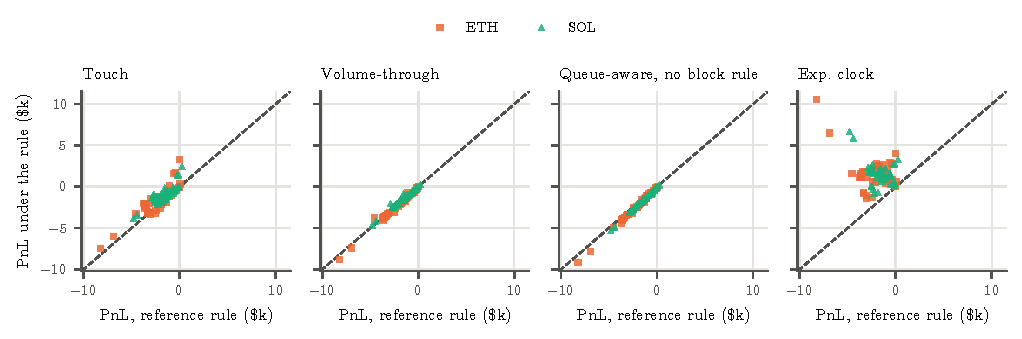
\includegraphics[width=\textwidth]{pnl_by_rule}}{\tbd}
\caption{Total PnL of each of the 48 strategy variants under a fill rule (vertical)
against its PnL under the reference rule (horizontal), 1~December 2025, before
fees. On the diagonal a rule agrees with the reference; above it, it flatters the
strategy.}
\label{fig:pnl}
\end{figure*}

\paragraph{Under the reference rule almost every strategy loses.}
Under \qa{} with the block rule, 47 of the 48 variants lose money before fees on
\ETH{} and 47 on \SOL{} (\BTC: \tbd). The only exceptions are a trade filter that
stands aside for five seconds after every trade on its side (\$48 on \ETH) and the
imbalance quoter deciding ten times a second (\$251 on \SOL); both trade little.
The four strategies of the original design lose on both instruments, and their
fills lose 1.25--1.64\bps{} one second later: a passive quote that reacts once a
second is filled mostly when the price is about to move through it. Fees would
deepen every loss.

\paragraph{\touch{} hides adverse selection.}
Under \touch{} the four original strategies fill 1.5 to 3 times as often as under
the reference (symmetric quoting: 40\,815 fills against 17\,110 on \SOL{} and
68\,166 against 23\,033 on \ETH), and their fills look far less toxic: one-second
markouts of $-0.15$ to $-1.17$\bps{} against $-1.25$ to $-1.64$. The extra fills are
the orders that in reality wait behind the queue and are reached only when the
price runs through the level. Across all 48 variants \touch{} flatters 92\% on
\SOL{} and 75\% on \ETH{} (Table~\ref{tab:ranking}, Figure~\ref{fig:pnl}), and
ranks them only loosely as the reference does ($\tau=0.59$ and $0.74$); on \ETH{}
only two of the reference's five best variants remain among its five best. The
most striking case is the imbalance quoter deciding ten times a second: under the
reference it fills 2\,842 times on \ETH{} and loses \$6; under \touch{} it fills
41\,528 times and makes \$3\,268, the best result of any variant.

\paragraph{\clock{} reverses the sign.}
Under the exponential clock fills arrive independently of the price path, so they
carry no adverse selection. It flatters every one of the 48 variants on both
instruments and turns 88\% of them from a loss into a profit; its ranking is
unrelated to the reference ($\tau=-0.20$ on \SOL, $-0.08$ on \ETH). The best
strategy under the clock is the five-level ladder, the \emph{worst} under the
reference: $-\$8\,230$ becomes $+\$10\,551$ on \ETH{} and $-\$4\,806$ becomes
$+\$6\,642$ on \SOL. The more orders a strategy rests, the more random fills the
clock grants it. The clock does not misprice adverse selection; it removes it.

\paragraph{\vt{} and the block rule.}
\vt{} ranks the variants almost as the reference does ($\tau=0.91$ and $0.96$,
all five best kept): it waits for more volume than in reality has to trade, but
the fills it grants are as toxic as the real ones. Its level differs by
instrument---it flatters 75\% of variants on \SOL{} but 6\% on \ETH. Removing the
block rule from \qa{} flatters none of the 48 variants: the fills that an in-block
cancellation prevents are, as in Section~\ref{sec:block}, the toxic ones, so
ignoring the exchange's processing order never makes a strategy look better.

\paragraph{Which strategies the rules favour.}
The rules' errors are not spread evenly. \touch{} favours most the strategies that
join the best price whatever its queue---imbalance, penny, sticky, symmetric and
skew quoters gain a median \$0.9--2.2k over the day---and favours least those
that stay away from long queues or quote deeper: offset, short-queue, A--S and
GLFT quoters gain $-\$0.6$k to $+\$0.2$k. The clock favours most the strategies
that rest the most orders: ladders gain a median \$11--16k. A backtest under
either rule therefore does not merely shift all strategies by a common amount; it
selects for a particular style of quoting.

\paragraph{Reaction speed.}
Under the reference rule, deciding faster helps the strategies that withdraw
quotes when the market turns: from five seconds to a tenth of a second the A--S
quoter's loss on \SOL{} falls from \$1\,136 to \$437, and the imbalance quoter
turns profitable on \SOL{} and breaks even on \ETH. It hurts the symmetric quoter, which only chases the best price
and so collects more fills of the same quality ($-\$2\,000$ to $-\$2\,891$). Under
the clock every strategy gains from speed, because more orders mean more random
fills. On \BTC: \tbd.

\paragraph{Sharpe ratio.} \tbd
